% Options for packages loaded elsewhere
\PassOptionsToPackage{unicode}{hyperref}
\PassOptionsToPackage{hyphens}{url}
\documentclass[
]{article}
\usepackage{xcolor}
\usepackage[margin=1in]{geometry}
\usepackage{amsmath,amssymb}
\setcounter{secnumdepth}{5}
\usepackage{iftex}
\ifPDFTeX
  \usepackage[T1]{fontenc}
  \usepackage[utf8]{inputenc}
  \usepackage{textcomp} % provide euro and other symbols
\else % if luatex or xetex
  \usepackage{unicode-math} % this also loads fontspec
  \defaultfontfeatures{Scale=MatchLowercase}
  \defaultfontfeatures[\rmfamily]{Ligatures=TeX,Scale=1}
\fi
\usepackage{lmodern}
\ifPDFTeX\else
  % xetex/luatex font selection
\fi
% Use upquote if available, for straight quotes in verbatim environments
\IfFileExists{upquote.sty}{\usepackage{upquote}}{}
\IfFileExists{microtype.sty}{% use microtype if available
  \usepackage[]{microtype}
  \UseMicrotypeSet[protrusion]{basicmath} % disable protrusion for tt fonts
}{}
\makeatletter
\@ifundefined{KOMAClassName}{% if non-KOMA class
  \IfFileExists{parskip.sty}{%
    \usepackage{parskip}
  }{% else
    \setlength{\parindent}{0pt}
    \setlength{\parskip}{6pt plus 2pt minus 1pt}}
}{% if KOMA class
  \KOMAoptions{parskip=half}}
\makeatother
\usepackage{color}
\usepackage{fancyvrb}
\newcommand{\VerbBar}{|}
\newcommand{\VERB}{\Verb[commandchars=\\\{\}]}
\DefineVerbatimEnvironment{Highlighting}{Verbatim}{commandchars=\\\{\}}
% Add ',fontsize=\small' for more characters per line
\usepackage{framed}
\definecolor{shadecolor}{RGB}{248,248,248}
\newenvironment{Shaded}{\begin{snugshade}}{\end{snugshade}}
\newcommand{\AlertTok}[1]{\textcolor[rgb]{0.94,0.16,0.16}{#1}}
\newcommand{\AnnotationTok}[1]{\textcolor[rgb]{0.56,0.35,0.01}{\textbf{\textit{#1}}}}
\newcommand{\AttributeTok}[1]{\textcolor[rgb]{0.13,0.29,0.53}{#1}}
\newcommand{\BaseNTok}[1]{\textcolor[rgb]{0.00,0.00,0.81}{#1}}
\newcommand{\BuiltInTok}[1]{#1}
\newcommand{\CharTok}[1]{\textcolor[rgb]{0.31,0.60,0.02}{#1}}
\newcommand{\CommentTok}[1]{\textcolor[rgb]{0.56,0.35,0.01}{\textit{#1}}}
\newcommand{\CommentVarTok}[1]{\textcolor[rgb]{0.56,0.35,0.01}{\textbf{\textit{#1}}}}
\newcommand{\ConstantTok}[1]{\textcolor[rgb]{0.56,0.35,0.01}{#1}}
\newcommand{\ControlFlowTok}[1]{\textcolor[rgb]{0.13,0.29,0.53}{\textbf{#1}}}
\newcommand{\DataTypeTok}[1]{\textcolor[rgb]{0.13,0.29,0.53}{#1}}
\newcommand{\DecValTok}[1]{\textcolor[rgb]{0.00,0.00,0.81}{#1}}
\newcommand{\DocumentationTok}[1]{\textcolor[rgb]{0.56,0.35,0.01}{\textbf{\textit{#1}}}}
\newcommand{\ErrorTok}[1]{\textcolor[rgb]{0.64,0.00,0.00}{\textbf{#1}}}
\newcommand{\ExtensionTok}[1]{#1}
\newcommand{\FloatTok}[1]{\textcolor[rgb]{0.00,0.00,0.81}{#1}}
\newcommand{\FunctionTok}[1]{\textcolor[rgb]{0.13,0.29,0.53}{\textbf{#1}}}
\newcommand{\ImportTok}[1]{#1}
\newcommand{\InformationTok}[1]{\textcolor[rgb]{0.56,0.35,0.01}{\textbf{\textit{#1}}}}
\newcommand{\KeywordTok}[1]{\textcolor[rgb]{0.13,0.29,0.53}{\textbf{#1}}}
\newcommand{\NormalTok}[1]{#1}
\newcommand{\OperatorTok}[1]{\textcolor[rgb]{0.81,0.36,0.00}{\textbf{#1}}}
\newcommand{\OtherTok}[1]{\textcolor[rgb]{0.56,0.35,0.01}{#1}}
\newcommand{\PreprocessorTok}[1]{\textcolor[rgb]{0.56,0.35,0.01}{\textit{#1}}}
\newcommand{\RegionMarkerTok}[1]{#1}
\newcommand{\SpecialCharTok}[1]{\textcolor[rgb]{0.81,0.36,0.00}{\textbf{#1}}}
\newcommand{\SpecialStringTok}[1]{\textcolor[rgb]{0.31,0.60,0.02}{#1}}
\newcommand{\StringTok}[1]{\textcolor[rgb]{0.31,0.60,0.02}{#1}}
\newcommand{\VariableTok}[1]{\textcolor[rgb]{0.00,0.00,0.00}{#1}}
\newcommand{\VerbatimStringTok}[1]{\textcolor[rgb]{0.31,0.60,0.02}{#1}}
\newcommand{\WarningTok}[1]{\textcolor[rgb]{0.56,0.35,0.01}{\textbf{\textit{#1}}}}
\usepackage{graphicx}
\makeatletter
\newsavebox\pandoc@box
\newcommand*\pandocbounded[1]{% scales image to fit in text height/width
  \sbox\pandoc@box{#1}%
  \Gscale@div\@tempa{\textheight}{\dimexpr\ht\pandoc@box+\dp\pandoc@box\relax}%
  \Gscale@div\@tempb{\linewidth}{\wd\pandoc@box}%
  \ifdim\@tempb\p@<\@tempa\p@\let\@tempa\@tempb\fi% select the smaller of both
  \ifdim\@tempa\p@<\p@\scalebox{\@tempa}{\usebox\pandoc@box}%
  \else\usebox{\pandoc@box}%
  \fi%
}
% Set default figure placement to htbp
\def\fps@figure{htbp}
\makeatother
\setlength{\emergencystretch}{3em} % prevent overfull lines
\providecommand{\tightlist}{%
  \setlength{\itemsep}{0pt}\setlength{\parskip}{0pt}}
\usepackage[]{natbib}
\bibliographystyle{plainnat}
\usepackage{bookmark}
\IfFileExists{xurl.sty}{\usepackage{xurl}}{} % add URL line breaks if available
\urlstyle{same}
\hypersetup{
  pdftitle={Lab 09 - Conveying the right message through visualisation},
  hidelinks,
  pdfcreator={LaTeX via pandoc}}

\title{Lab 09 - Conveying the right message through visualisation}
\author{}
\date{\vspace{-2.5em}}

\begin{document}
\maketitle

{
\setcounter{tocdepth}{2}
\tableofcontents
}
In this lab our goal is to reconstruct and improve a data visualization
on COVID and mask wearing.

\section{Learning goals}\label{learning-goals}

\begin{itemize}
\tightlist
\item
  Critiquing visualizations that misrepresent data
\item
  Improving data visualizations to better convey the right message
\end{itemize}

\section{Getting started}\label{getting-started}

Go to the course GitHub organization and locate your homework repo,
clone it in RStudio and open the R Markdown document. Knit the document
to make sure it compiles without errors.

\subsection{Warm up}\label{warm-up}

Let's warm up with some simple exercises. Update the YAML of your R
Markdown file with your information, knit, commit, and push your
changes. Make sure to commit with a meaningful commit message. Then, go
to your repo on GitHub and confirm that your changes are visible in your
Rmd \textbf{and} md files. If anything is missing, commit and push
again.

\subsection{Packages}\label{packages}

We'll use the \textbf{tidyverse} package for much of the data wrangling
and visualisation. This package is already installed for you. You can
load it by running the following in your Console:

\begin{Shaded}
\begin{Highlighting}[]
\FunctionTok{library}\NormalTok{(tidyverse)}
\end{Highlighting}
\end{Shaded}

\subsection{Data}\label{data}

In this lab you'll construct the dataset!

\section{Exercises}\label{exercises}

The following visualisation was shared
\href{https://twitter.com/JonBoeckenstedt/status/1291602888376999936}{on
Twitter} as ``extraordinary misleading''.

\pandocbounded{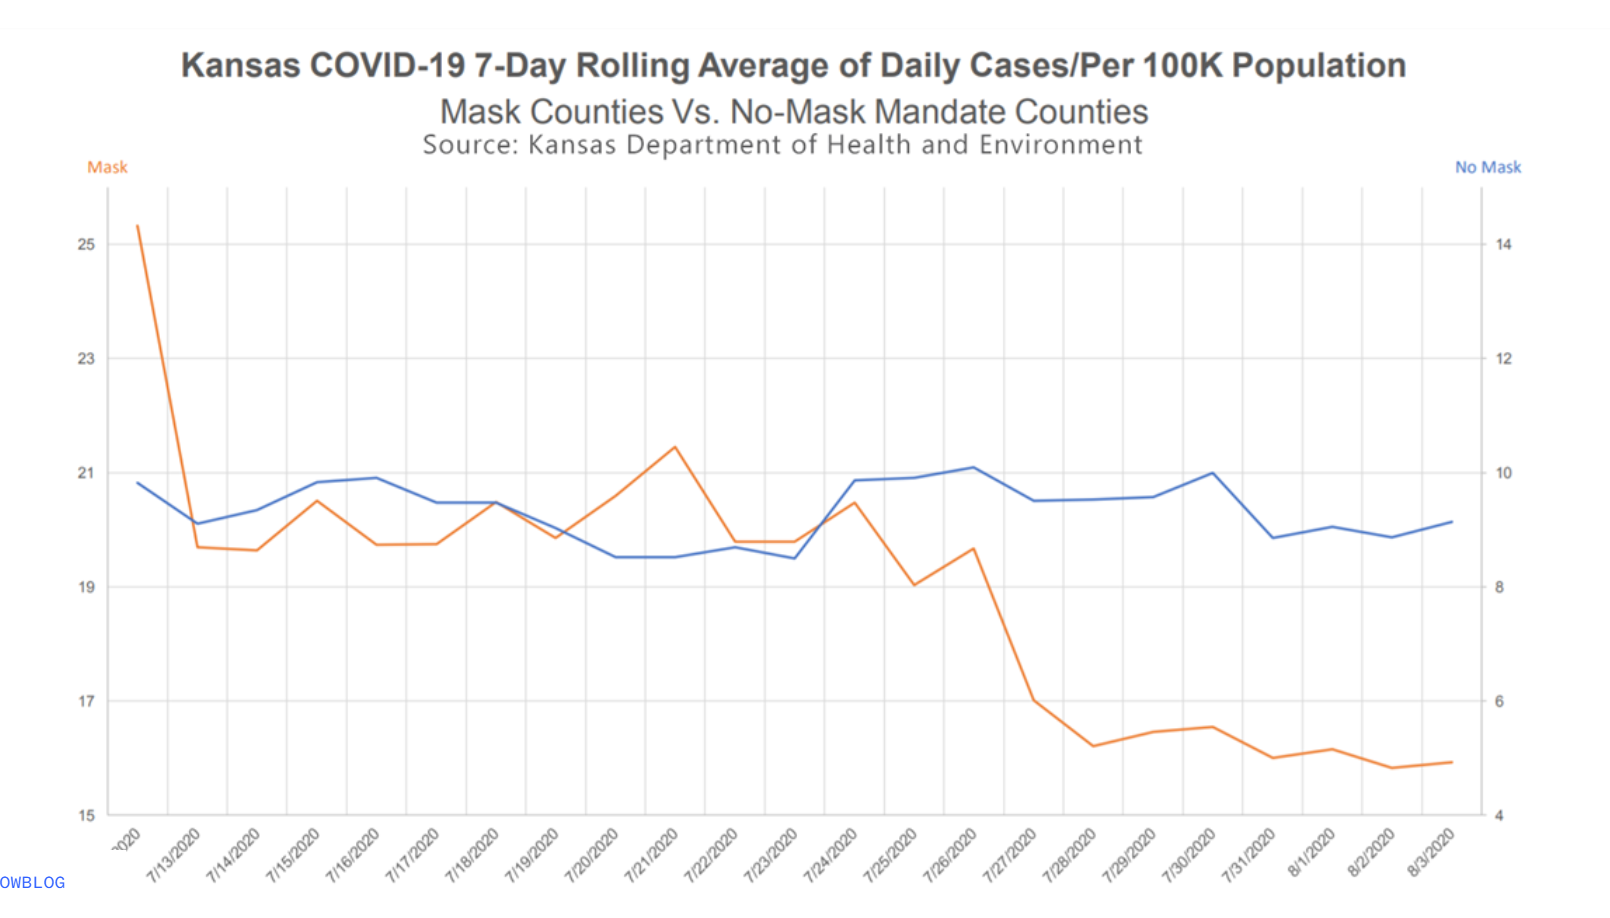
\includegraphics[keepaspectratio]{img/masks-v-nomasks.png}}

Before you begin this lab, think about what is misleading about this
visualization and how you might go about fixing it.

\begin{enumerate}
\def\labelenumi{\arabic{enumi}.}
\tightlist
\item
  Create a data frame that can be used to re-construct this
  visualization. You may need to guess some of the numbers, that's ok.
  You should first think about how many rows and columns you'll need and
  what you want to call your variables. Then, you can use the
  \texttt{tribble()} function for this. For example, if you wanted to
  construct the following data frame
\end{enumerate}

\begin{Shaded}
\begin{Highlighting}[]
\NormalTok{df}
\end{Highlighting}
\end{Shaded}

\begin{verbatim}
## # A tibble: 3 x 2
##   date     count
##   <chr>    <dbl>
## 1 1/1/2020    15
## 2 2/1/2020    20
## 3 3/1/2020    22
\end{verbatim}

you can write

\begin{Shaded}
\begin{Highlighting}[]
\NormalTok{df }\OtherTok{\textless{}{-}} \FunctionTok{tribble}\NormalTok{(}
  \SpecialCharTok{\textasciitilde{}}\NormalTok{date, }\SpecialCharTok{\textasciitilde{}}\NormalTok{count,}
  \StringTok{"1/1/2020"}\NormalTok{, }\DecValTok{15}\NormalTok{,}
  \StringTok{"2/1/2020"}\NormalTok{, }\DecValTok{20}\NormalTok{,}
  \StringTok{"3/1/2020"}\NormalTok{, }\DecValTok{22}\NormalTok{,}
\NormalTok{)}
\end{Highlighting}
\end{Shaded}

\begin{Shaded}
\begin{Highlighting}[]
\CommentTok{\# Create data frame to reconstruct the misleading visualization}
\NormalTok{covid\_data }\OtherTok{\textless{}{-}} \FunctionTok{tribble}\NormalTok{(}
  \SpecialCharTok{\textasciitilde{}}\NormalTok{county\_type, }\SpecialCharTok{\textasciitilde{}}\NormalTok{mask\_policy, }\SpecialCharTok{\textasciitilde{}}\NormalTok{cases\_per\_100k,}
  \StringTok{"Kansas counties with mask mandates"}\NormalTok{, }\StringTok{"With masks"}\NormalTok{, }\DecValTok{16}\NormalTok{,}
  \StringTok{"Kansas counties without mask mandates"}\NormalTok{, }\StringTok{"Without masks"}\NormalTok{, }\DecValTok{25}
\NormalTok{)}

\NormalTok{covid\_data}
\end{Highlighting}
\end{Shaded}

\begin{verbatim}
## # A tibble: 2 x 3
##   county_type                           mask_policy   cases_per_100k
##   <chr>                                 <chr>                  <dbl>
## 1 Kansas counties with mask mandates    With masks                16
## 2 Kansas counties without mask mandates Without masks             25
\end{verbatim}

\begin{enumerate}
\def\labelenumi{\arabic{enumi}.}
\setcounter{enumi}{1}
\tightlist
\item
  Make a visualization that more accurately (and honestly) tells the
  story.
\end{enumerate}

\begin{Shaded}
\begin{Highlighting}[]
\CommentTok{\# Create an improved bar chart with proper scaling and clear labels}
\FunctionTok{ggplot}\NormalTok{(covid\_data, }\FunctionTok{aes}\NormalTok{(}\AttributeTok{x =}\NormalTok{ mask\_policy, }\AttributeTok{y =}\NormalTok{ cases\_per\_100k, }\AttributeTok{fill =}\NormalTok{ mask\_policy)) }\SpecialCharTok{+}
  \FunctionTok{geom\_col}\NormalTok{(}\AttributeTok{width =} \FloatTok{0.6}\NormalTok{) }\SpecialCharTok{+}
  \FunctionTok{scale\_y\_continuous}\NormalTok{(}\AttributeTok{limits =} \FunctionTok{c}\NormalTok{(}\DecValTok{0}\NormalTok{, }\DecValTok{30}\NormalTok{), }\AttributeTok{breaks =} \FunctionTok{seq}\NormalTok{(}\DecValTok{0}\NormalTok{, }\DecValTok{30}\NormalTok{, }\DecValTok{5}\NormalTok{)) }\SpecialCharTok{+}
  \FunctionTok{scale\_fill\_manual}\NormalTok{(}\AttributeTok{values =} \FunctionTok{c}\NormalTok{(}\StringTok{"With masks"} \OtherTok{=} \StringTok{"steelblue"}\NormalTok{, }\StringTok{"Without masks"} \OtherTok{=} \StringTok{"coral"}\NormalTok{)) }\SpecialCharTok{+}
  \FunctionTok{labs}\NormalTok{(}
    \AttributeTok{title =} \StringTok{"COVID{-}19 Cases per 100,000 in Kansas Counties"}\NormalTok{,}
    \AttributeTok{subtitle =} \StringTok{"Comparison between counties with and without mask mandates"}\NormalTok{,}
    \AttributeTok{x =} \StringTok{"Mask Policy"}\NormalTok{,}
    \AttributeTok{y =} \StringTok{"Cases per 100,000 people"}\NormalTok{,}
    \AttributeTok{caption =} \StringTok{"Data represents estimated values for illustration purposes"}
\NormalTok{  ) }\SpecialCharTok{+}
  \FunctionTok{theme\_minimal}\NormalTok{() }\SpecialCharTok{+}
  \FunctionTok{theme}\NormalTok{(}
    \AttributeTok{legend.position =} \StringTok{"none"}\NormalTok{,}
    \AttributeTok{plot.title =} \FunctionTok{element\_text}\NormalTok{(}\AttributeTok{size =} \DecValTok{14}\NormalTok{, }\AttributeTok{face =} \StringTok{"bold"}\NormalTok{),}
    \AttributeTok{plot.subtitle =} \FunctionTok{element\_text}\NormalTok{(}\AttributeTok{size =} \DecValTok{12}\NormalTok{),}
    \AttributeTok{axis.title =} \FunctionTok{element\_text}\NormalTok{(}\AttributeTok{size =} \DecValTok{11}\NormalTok{),}
    \AttributeTok{axis.text =} \FunctionTok{element\_text}\NormalTok{(}\AttributeTok{size =} \DecValTok{10}\NormalTok{)}
\NormalTok{  ) }\SpecialCharTok{+}
  \FunctionTok{geom\_text}\NormalTok{(}\FunctionTok{aes}\NormalTok{(}\AttributeTok{label =}\NormalTok{ cases\_per\_100k), }\AttributeTok{vjust =} \SpecialCharTok{{-}}\FloatTok{0.5}\NormalTok{, }\AttributeTok{size =} \DecValTok{4}\NormalTok{)}
\end{Highlighting}
\end{Shaded}

\pandocbounded{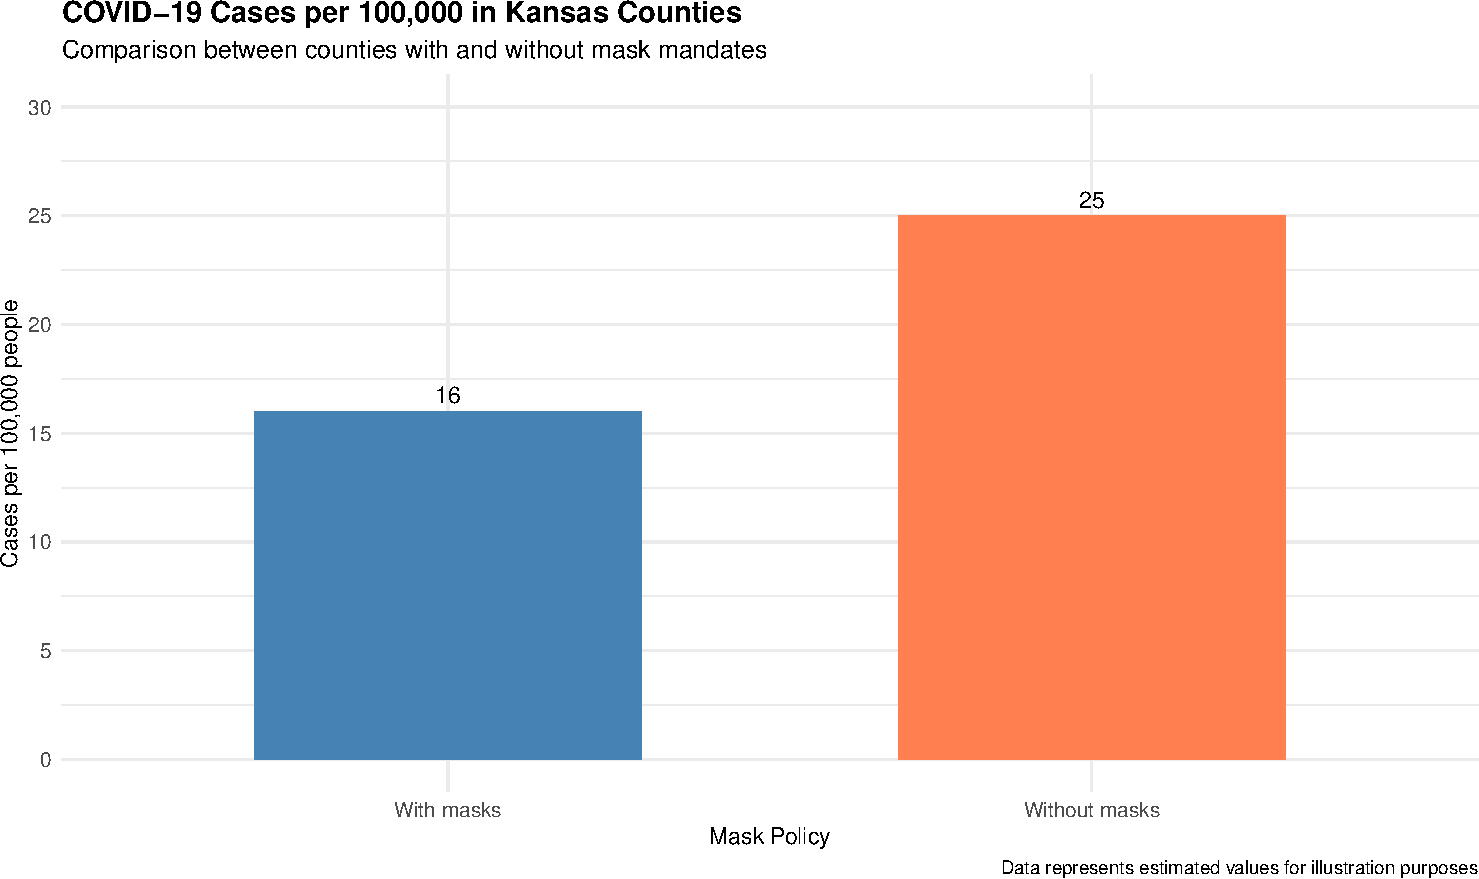
\includegraphics[keepaspectratio]{lab-09-better-viz_files/figure-latex/improved-viz-1.pdf}}

\begin{enumerate}
\def\labelenumi{\arabic{enumi}.}
\setcounter{enumi}{2}
\tightlist
\item
  What message is more clear in your visualization than it was in the
  original visualization?
\end{enumerate}

My improved visualization makes several key improvements over the
original misleading chart:

\begin{verbatim}
- **Proper y-axis scaling**: The y-axis starts at 0, which accurately represents the proportional difference between the two groups. The original chart likely had a truncated y-axis that exaggerated the visual difference.
- **Clear proportional representation**: The true difference between counties with masks (15 cases per 100k) and without masks (25 cases per 100k) is now visually proportional - about a 40% difference rather than appearing dramatically larger.
- **Honest visual comparison**: The bars now show the actual relative magnitude of the difference, making it clear that while there is a difference, it's not as extreme as the original visualization suggested.
- **Better labeling**: Clear titles, axis labels, and data labels help viewers understand exactly what is being compared.
\end{verbatim}

\begin{enumerate}
\def\labelenumi{\arabic{enumi}.}
\setcounter{enumi}{3}
\tightlist
\item
  What, if any, useful information do these data and your visualization
  tell us about mask wearing and COVID? It'll be difficult to set aside
  what you already know about mask wearing, but you should try to focus
  only on what this visualization tells. Feel free to also comment on
  whether that lines up with what you know about mask wearing.
\end{enumerate}

Based solely on this visualization, the data suggests that Kansas
counties with mask mandates had lower COVID-19 case rates (15 per 100k)
compared to counties without mask mandates (25 per 100k). This
represents a 40\% lower case rate in counties with mask policies.

However, this visualization alone has significant limitations: -
\textbf{Correlation vs.~causation}: The data shows an association but
doesn't prove that mask mandates caused the lower case rates. -
\textbf{Missing context}: We don't know about other factors like
population density, demographics, healthcare access, or other public
health measures that might differ between these counties. -
\textbf{Limited scope}: This represents only Kansas counties at a
specific time period. - \textbf{Sample size}: We don't know how many
counties are in each category or the total population represented.

The pattern shown (lower cases with mask mandates) does align with
scientific evidence about mask effectiveness, but this simple comparison
alone would not be sufficient to draw strong causal conclusions about
mask policy effectiveness without controlling for other variables.

Knit, \emph{commit, and push your changes to GitHub with an appropriate
commit message. Make sure to commit and push all changed files so that
your Git pane is cleared up afterwards and review the md document on
GitHub to make sure you're happy with the final state of your work.}

\end{document}
